\chapter{Theory}

Let us show an example of figure insertion here
\begin{figure}
	\center
	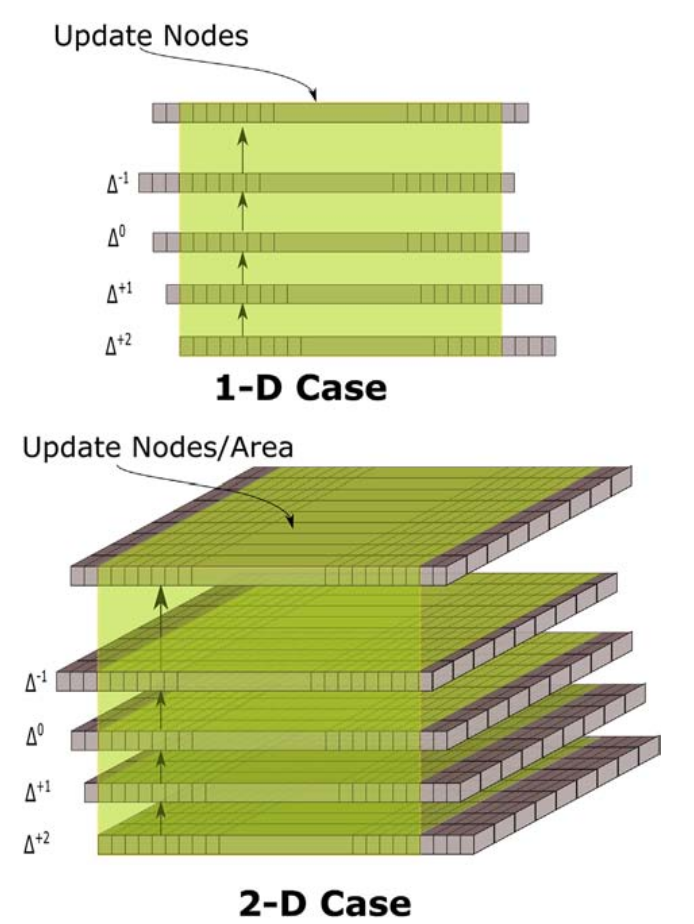
\includegraphics[width=.6\textwidth]{theory_vectorize_operator.png}
	\caption{The figure is taken from  \cite{malkoti_algorithm_2018} 
	to show how to include a figure. 
	A uniquie lable  is attached to this figure so that it can be 
	referred anywhere in the thesis.}
	\label{fig:theory_vectorize}
\end{figure}




The figure can be cited anywhere in the text using the ref command 
for example  Figure \ref{fig:theory_vectorize}

However a better choice in some cases might be the new command provided by the package 
see \reftablet{tab:list_ref_cmd}.  

%
\begin{table}
\caption{ List of new commands provided by this package}
\label{tab:list_ref_cmd}
\center
\begin{tabular}{cc}
	\hline
	\verb|reffig{fig:theory_vectorize} |		&	\reffig{fig:theory_vectorize} 	\\
	\verb|reffigt{fig:theory_vectorize}|		&	\reffigt{fig:theory_vectorize}	\\
	\verb|reffigp{fig:theory_vectorize}|		& 	\reffigp{fig:theory_vectorize}	\\
	\verb|reftable{tab:citation_style} |		&	\reftable{tab:citation_style} \\
	\verb|reftablet{tab:citation_style}|		&	\reftablet{tab:citation_style}	\\
	\verb|reftablep{tab:citation_style}|		&  	\reftablep{tab:citation_style} \\
	\hline
\end{tabular}
\end{table} 

 
  